\documentclass[11pt]{article}
\input{Preambulo/paquetes}

%---------------- INICIO DEL DOCUMENTO ----------------%
\begin{document}
\input{Preambulo/Variables}
%-------------------- PORTADA --------------------%
\input{Preambulo/portada}
\newpage

%-------------------- INDICES --------------------%
\newpage
\pagestyle{empty}
\renewcommand{\contentsname}{{\huge Índice}}
\tableofcontents

%---------------- DESARROLLO ----------------%
\lhead{\the\materia}
\chead{
\includegraphics[scale=0.02]{Imagenes/LOGO ITBA.png}}
\rhead{\the\grupo}

%---------------- Info de Pagina ----------------%
\newpage
\pagestyle{fancy} %activa encabezado y pie de pagina

\setcounter{page}{1} %empezar numeración desde está pagina
\setcounter{equation}{0} %empezar numeración desde 1 para ecuaciones
\setcounter{figure}{0} %empezar numeración desde 1 para figuras
\setcounter{table}{0} %empezar numeración desde 1 para tablas

%\label{sec: label de la seccion} %los labels tambien funcionan con secciones

%---------------- Introducción ---------------%
\section{Introducción}
En el presente trabajo se estudiará el diseño de circuitos digitales utilizando la tecnología CMOS.
Se utilizará la simulación para analizar las diferencias entre los cálculos teóricos y los resultados
obtenidos en la práctica.

%---------------- 1ra Seccion ----------------%
\section{Compuerta NOT}
\label{sec:compuerta not}
Dado el circuito de la compuerta NOT se pide que $V_{sp}$ (Inverter Switching Voltage) = $\frac{V_{DD}}{2}$.

Para ello se necesita que se cumpla la condición, asumiendo que ambos se encuentran en saturación:
\begin{equation}
    \frac{1}{2} \cdot K_{p_n} \cdot \frac{W_n}{L_n} \cdot (V_{sp} - V_{th_n})^2 = \frac{1}{2} \cdot K_{p_p} \cdot \frac{W_p}{L_p} \cdot (V_{DD} - V_{sp} - |V_{th_p}|)^2
\end{equation}

Despejando $V_{sp}$ se puede expresar como:

\begin{equation}
    V_{sp} = \frac{\sqrt {\frac{\beta_n}{\beta_p}}\cdot V_{th_n} + V_{DD} - V_{th_p}}{1+\sqrt{\frac{\beta_n}{\beta_p}}}
\end{equation}

Donde $\beta_n = \frac{1}{2}K_{p_n} \cdot \frac{W_n}{L_n}$ y $\beta_p = \frac{1}{2}K_{p_p} \cdot \frac{W_p}{L_p}$.

\subsection{Ancho de PMOS - Teórico}

Por ende, considerando que $V_{sp} = \frac{V_{DD}}{2}$ y asumiendo que $V_{th_n} = |V_{th_p}|$ se requiere que:

\begin{equation}
    K_{p_n}\cdot \frac{W_n}{L_n} = K_{p_p} \cdot \frac{W_p}{L_p}
\end{equation}

Con las siguientes restricciones:
\begin{itemize}
    \item $L_n = 1 \mu m$
    \item $L_p = 1 \mu m$
    \item $K_{p_n} = 120 \mu A/V^2$
    \item $K_{p_p} = 40 \mu A/V^2$
    \item $W_n = 2 \mu m$
\end{itemize}

$ W_p = 3\cdot W_n = 6 \mu m $

\subsection{Ancho de PMOS - Simulación}

Se simuló el circuito utilizando el software LTSpice y se obtuvo que el ancho necesario para que $V_{sp} = \frac{V_{DD}}{2}$ no 
se corresponde con la predicción teórica con mucha presición ya que mediante prueba y error en la simulación, partiendo del valor
teórico, se obtuvo que el ancho necesario para el PMOS es de $W_p \approx 4.83 \mu m$.



%---------------- 2da Seccion ----------------%
\section{Layout NOT}
\begin{figure}[h]
    \centering
    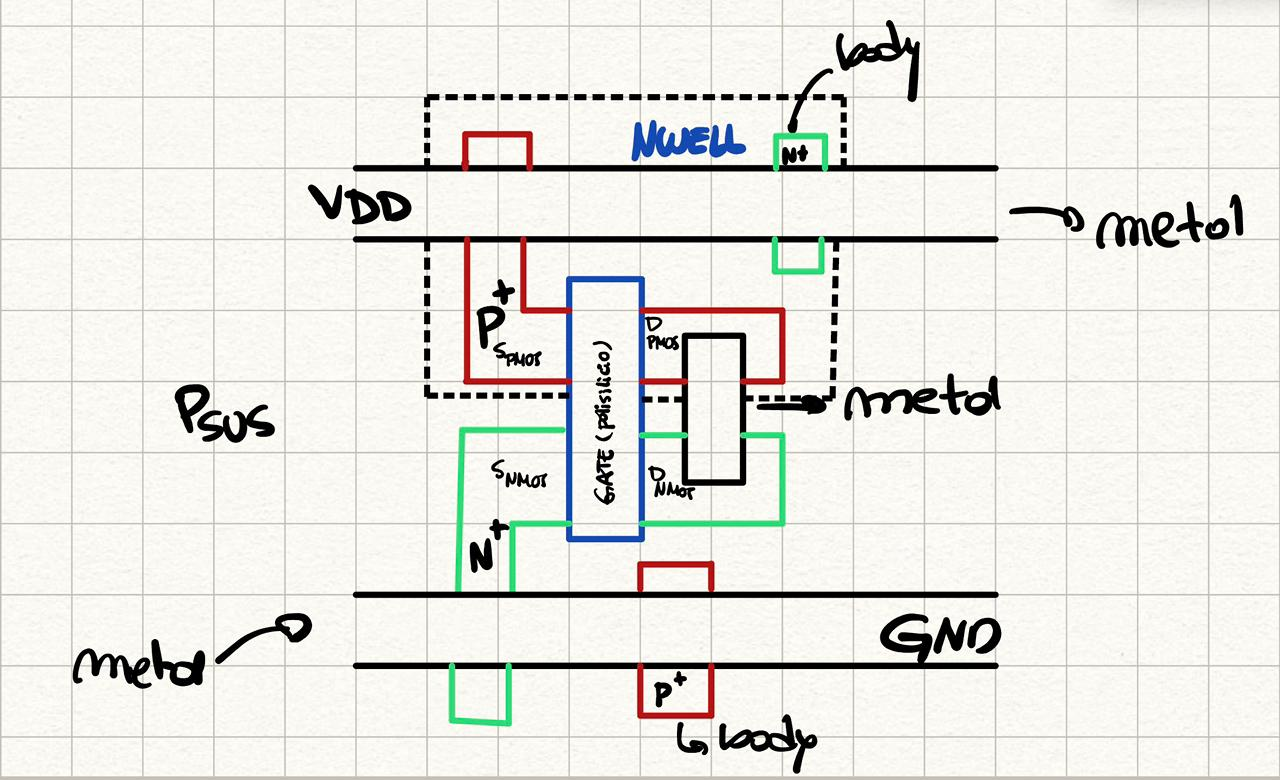
\includegraphics[width=0.5\textwidth]{Imagenes/Layout NOT.jpeg}
    \caption{Layout de la compuerta NOT}
    \label{fig:layout not}
\end{figure}


%---------------- 3ra Seccion ----------------%
\section{Compuertas NOT - Variación de relación de $\beta$}
\subsection{Calculo de $W_{p}$ correspondiente a cada compuerta NOT}

Se definen tres compuertas NOT en cascada con las características:
\begin{itemize}
    \item $\frac{\beta_{n_1}}{\beta_{p_1}} = 1$
    \item $\frac{\beta_{n_2}}{\beta_{p_2}} = 10$
    \item $\frac{\beta_{n_3}}{\beta_{p_3}} = 0.1$
\end{itemize}

Donde los transistores de la primera compuerta son los mismos que los de la sección \ref{sec:compuerta not}.

Por ende, $W_n = 2 \mu m$ y $W_p = 4.83 \mu m$ para la primera compuerta, considerando la simulación realizada.
Y para las siguientes compuertas, considerando las modificaciones hechas a la primera, serán de $W_{p_2} = 0.483 \mu m$ y $W_{p_3} = 48.3 \mu m$.

\subsection{Simulación de las compuertas NOT}

\begin{figure}[H]
    \centering
    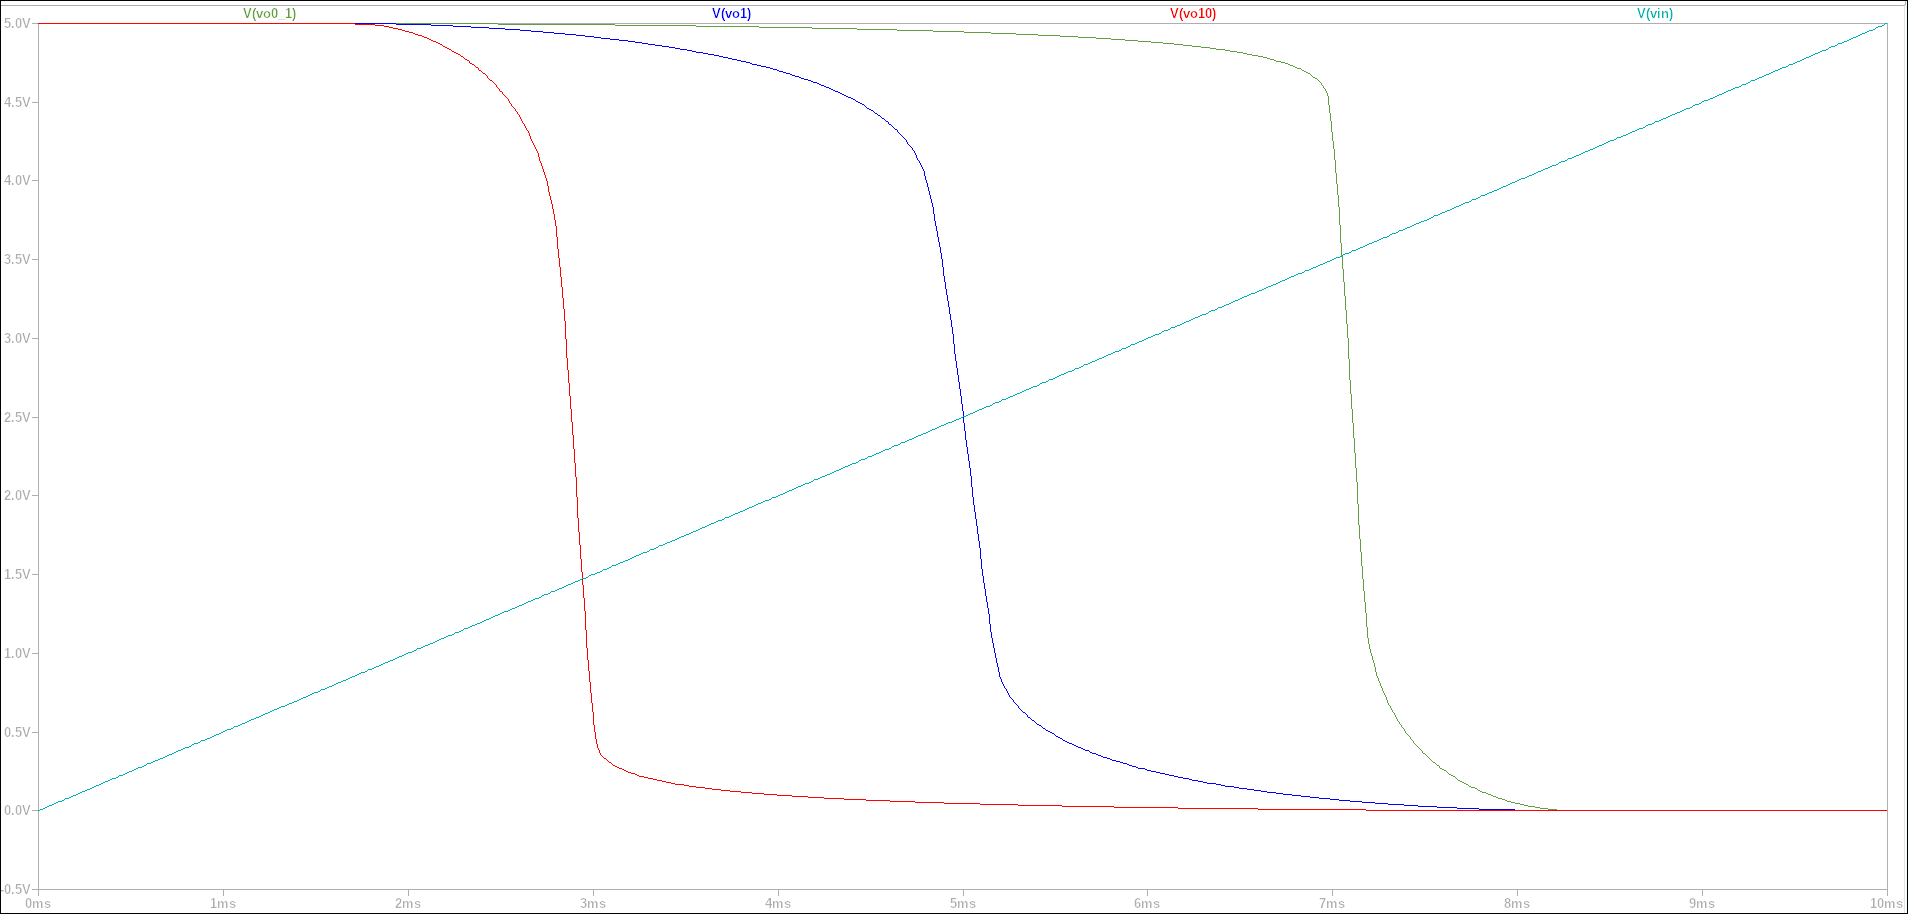
\includegraphics[width=0.8\textwidth]{Imagenes/ej3.png}
    \caption{Simulación de las compuertas NOT con diferentes relaciones $\frac{\beta_n}{\beta_p}$}
    \label{fig:not_simulation}
\end{figure}

\subsection{Márgenes de Ruido}
Los márgenes de ruido se pueden calcular a partir de las curvas de transferencia de las compuertas NOT. Para cada compuerta, se identifican los puntos donde la salida cambia de estado (de alto a bajo o viceversa) y se determinan los niveles de voltaje correspondientes.

\begin{equation}
    NMH = V_{OH} - V_{IH}
\end{equation}
\begin{equation}
    NML = V_{IL} - V_{OL}
\end{equation}

Los puntos de transición se obtienen de encontrar donde la derivada es de módulo unitario.

\begin{table}[H]
    \centering
    \begin{tabular}{l|c|c|c} \hline
    Relación $\frac{\beta_n}{\beta_p}$ & 1 & 10 & 0.1 \\ \hline
    NMH & 1.765 & 3.310 & 3.290 \\ 
    NML & 1.745 & 0.805 & 0.817 \\ \hline
    \end{tabular}
    \caption{Márgenes de ruido para cada compuerta NOT}
    \label{tab:margenes_ruido}
\end{table}

Se puede apreciar de la tabla que el margen de ruido es más simétrico cuánto más cercana a 1 es la relación $\frac{\beta_n}{\beta_p}$. 
Esto se debe a que una relación de 1 implica que los transistores NMOS y PMOS tienen características similares, lo que resulta en una curva de transferencia más equilibrada. 
En cambio, relaciones extremas (10 o 0.1) generan curvas de transferencia más asimétricas, lo que afecta negativamente los márgenes de ruido.


%---------------- 4ta Seccion ----------------%
\section{Tiempos de propagación}
\begin{figure}[H]
        \subfigure[Tiempo de LOW a HIGH]{
            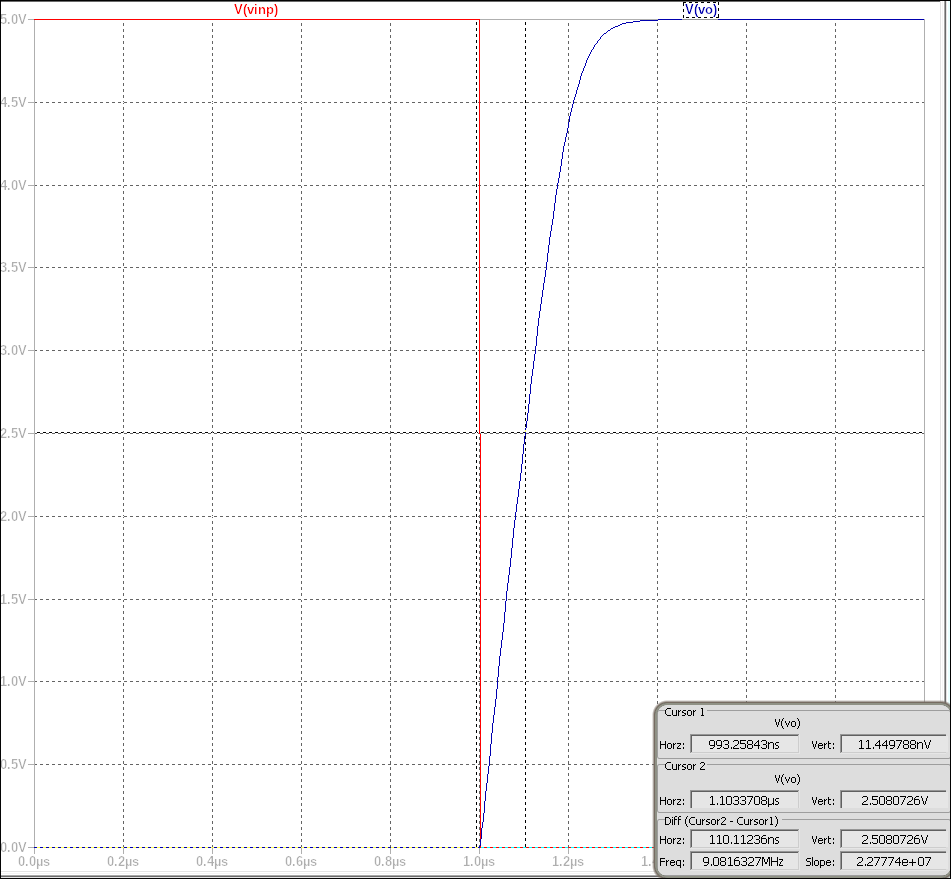
\includegraphics[width=.48\linewidth]{Imagenes/tL2H.png}
            \label{subfig:tL2H}
        }\hfill
        \subfigure[Tiempo de HIGH a LOW]{
            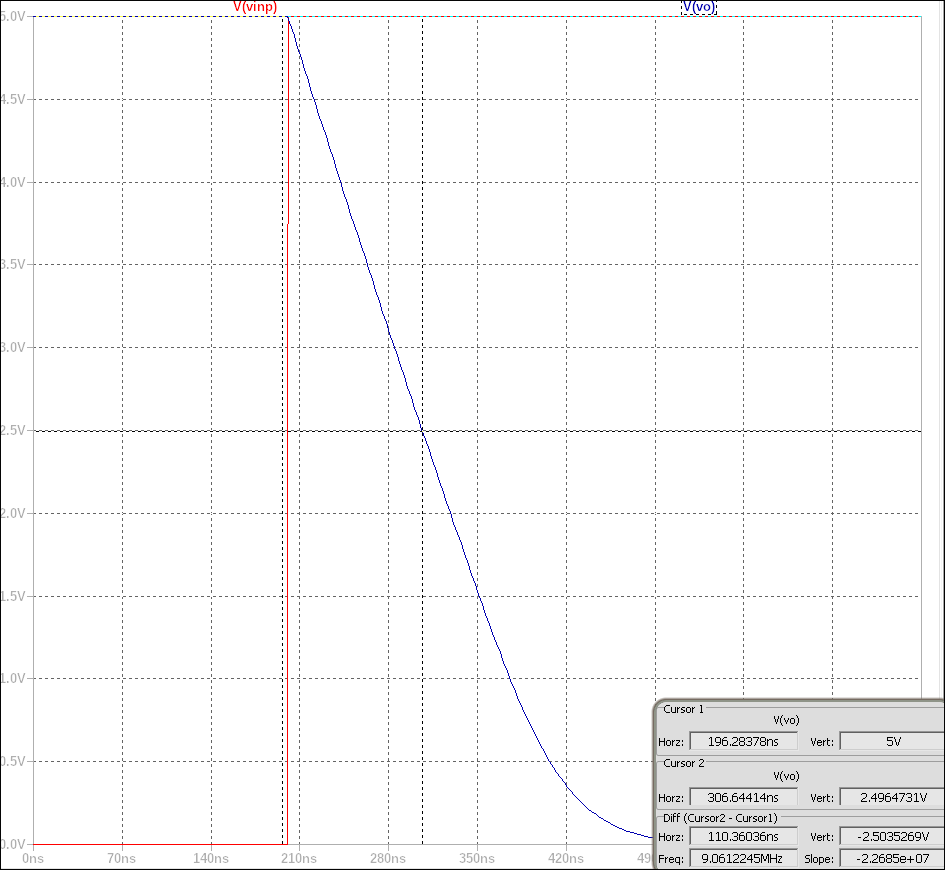
\includegraphics[width=.48\linewidth]{Imagenes/tH2L.png}
            \label{subfig:tH2L}
        }
        \caption{Tiempos de propagación para la compuerta NOT}
        \label{fig: tiempos_propagacion}
\end{figure}

Se puede observar que el tiempo de propagación de HIGH a LOW es de 110.36ns, similar al tiempo de LOW a HIGH que es de 110.1ns.



%---------------- 5ta Seccion ----------------%
\section{Tiempo de propagación con compuertas en serie}
Para analizar la conexión en serie, se utilizarán cinco compuertas con las siguientes característicsa:
\begin{itemize}
    \item $W_{n_2} = 2\cdot W_{n_1}$
    \item $W_{p_2} = 2\cdot W_{p_1}$
    \item $W_{n_3} = 4\cdot W_{n_1}$
    \item $W_{p_3} = 4\cdot W_{p_1}$
    \item $W_{n_4} = 8\cdot W_{n_1}$
    \item $W_{p_4} = 8\cdot W_{p_1}$
    \item $W_{n_5} = 16\cdot W_{n_1}$
    \item $W_{p_5} = 16\cdot W_{p_1}$
\end{itemize}

Es esperable que los tiempos de propagación aumenten a medida que se agregan compuertas en serie.
Sin embargo no se dió así la simulación.
\begin{figure}[H]
        \subfigure[Tiempo de LOW a HIGH]{
            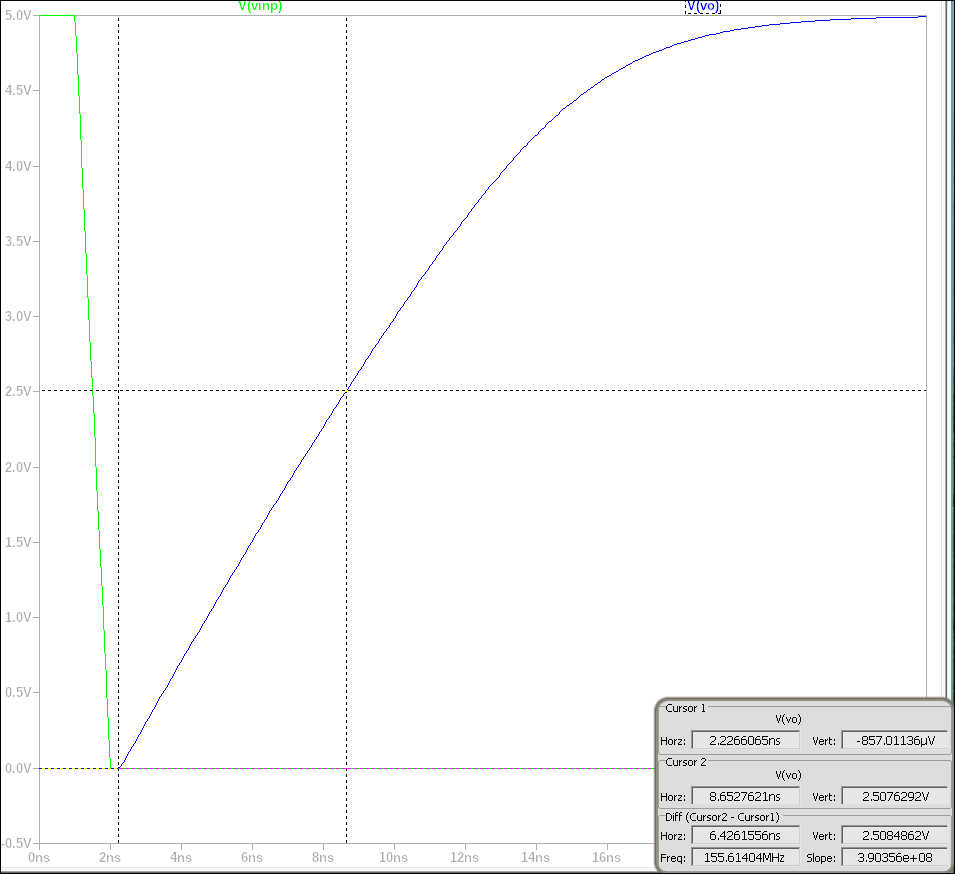
\includegraphics[width=.48\linewidth]{Imagenes/tL2HSerie.png}
            \label{subfig:tL2Hserie}
        }\hfill
        \subfigure[Tiempo de HIGH a LOW]{
            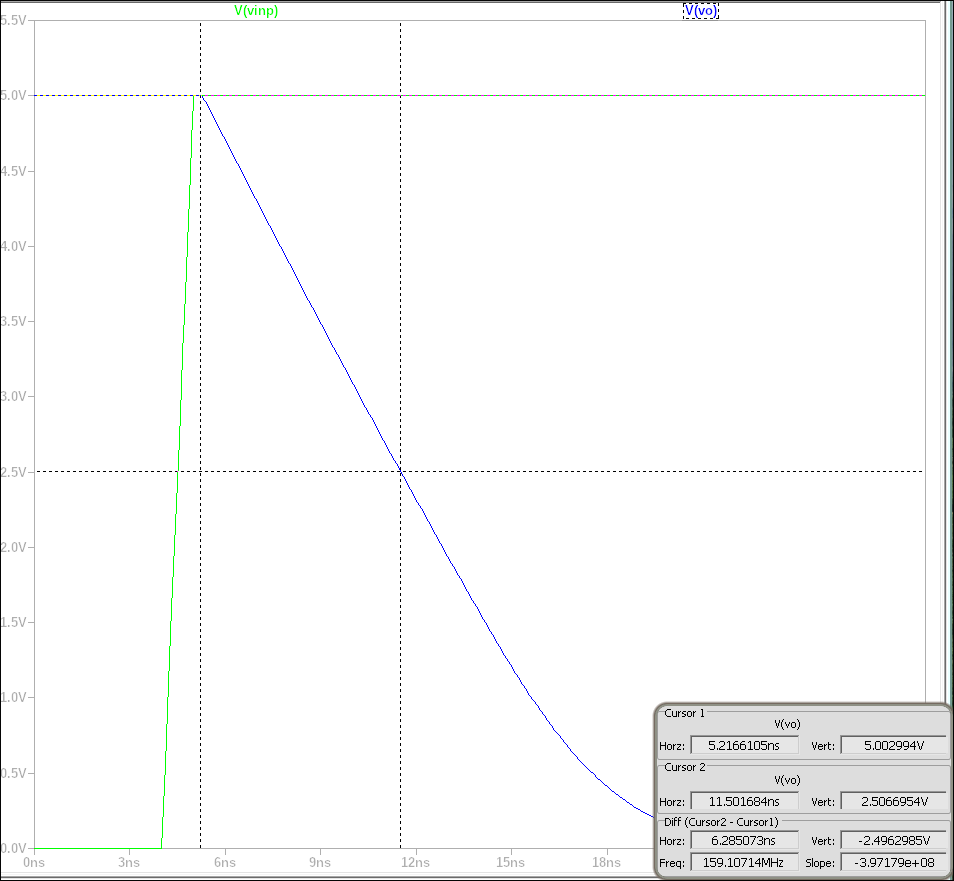
\includegraphics[width=.48\linewidth]{Imagenes/tH2LSerie.png}
            \label{subfig:tH2Lserie}
        }
        \caption{Tiempos de propagación para la compuerta NOT}
        \label{fig: tiempos_propagacionSerie}
\end{figure}
Esto se debe a que los anchos de las compuertas son diferentes entre si, donde la compuerta de mayor ancho se encuentra a la salida junto al capacitor.
Por eso el tiempo de propagación LOW to HIGH es de $t_{LtoH} = 6.43ns$ y el tiempo de propagación HIGH to LOW es de $t_{HtoL} = 6.28ns$. 
Los tiempos se mantuvieron cercanos entre sí debido a que los anchos de las compuertas mantuvieron la proporción de $\frac{\beta_n}{\beta_p}$.


%---------------- 6ta Seccion ----------------%
\section{Compuertas NAND y NOR}
Asumiendo que debido a igual proceso de fabricación, se cumple $V_{THn} = -V_{THp}$, se puede deducir a partir de los calculos de las resistencias de salida de las etapas de las compuertas.

\subsection{Compuerta NOR}
\begin{equation}
    \frac{\beta_n}{\beta_p} = \frac{k_{p_n}\frac{W_n}{2\cdot L_n}}{k_{p_p}\frac{W_p}{L_p}} = \frac{1}{2}
\end{equation}

Entonces para $W_n = 2 \mu m$, la condición impone $W_p = 12 \mu m$.

Esto produce la siguiente respuesta $V_{(V_{i})}$:

\begin{figure}[H]
    \centering
    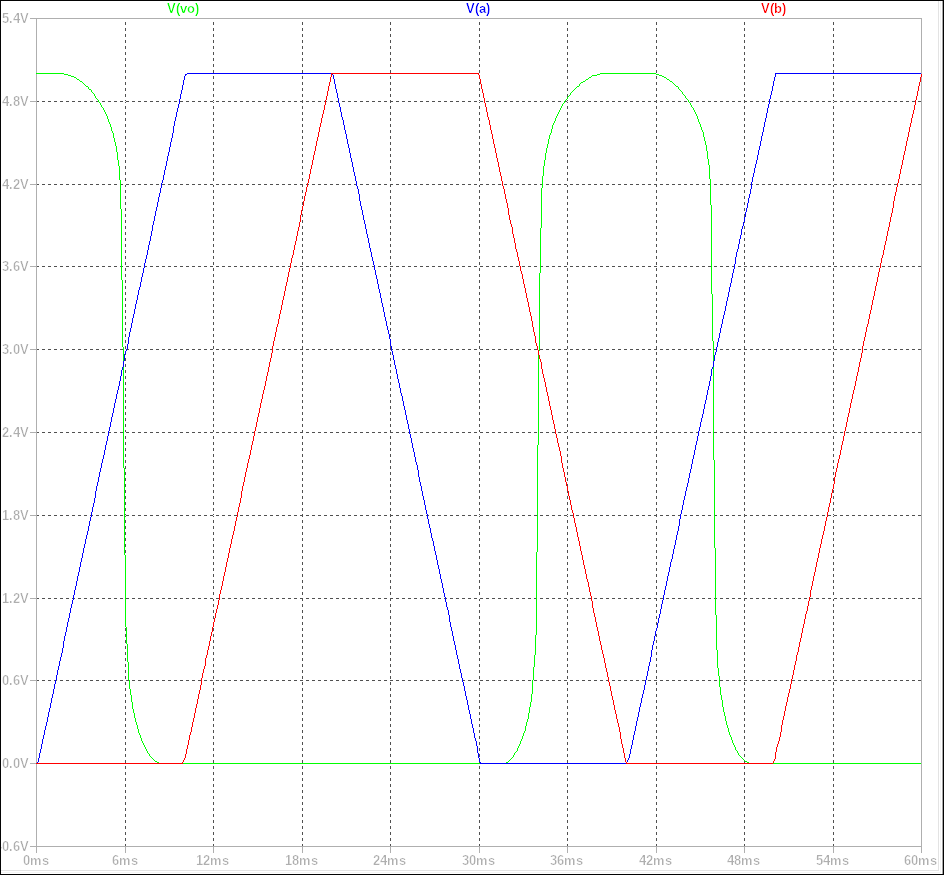
\includegraphics[width=0.8\textwidth]{Imagenes/NOR12u.png}
    \caption{Respuesta Celda NOR con $W_p = 12\mu m$}
    \label{fig:norChoto}
\end{figure}
Como se puede observar en la simulación este resultado implica que $V_{sp} \neq \frac{V_{DD}}{2}$.

Para esto se necesita $W_p \approx 6 \mu m$.
\begin{figure}[H]
    \centering
    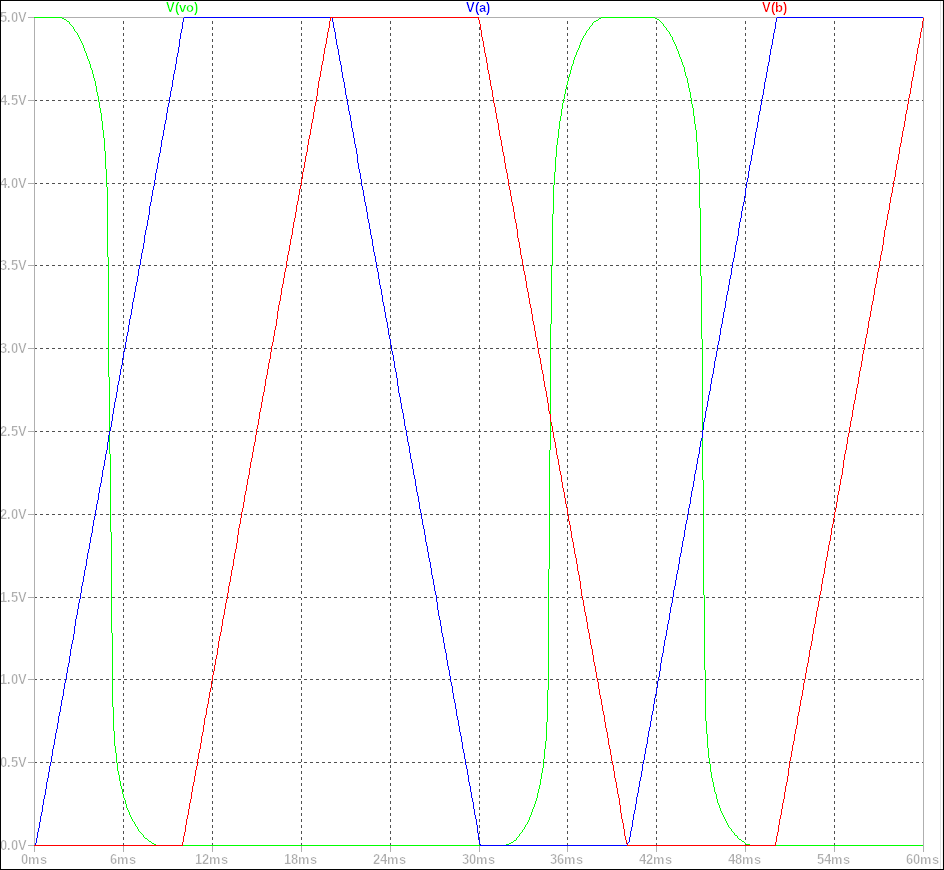
\includegraphics[width=0.8\textwidth]{Imagenes/NOR6u.png}
    \caption{Respuesta Celda NOR con $W_p \approx 6\mu m$}
    \label{fig:norBueno}
\end{figure}

\subsection{Compuerta NAND}
\begin{equation}
    \frac{\beta_n}{\beta_p} = \frac{k_{p_n}\frac{W_n}{L_n}}{k_{p_p}\frac{W_p}{2\cdot L_p}} = 2
\end{equation}

Entonces, con $W_n = 2\mu m$, la condición impone $W_p = 3 \mu m$.

Esto produce la siguiente respuesta $V_{(V_{i})}$:

\begin{figure}[H]
    \centering
    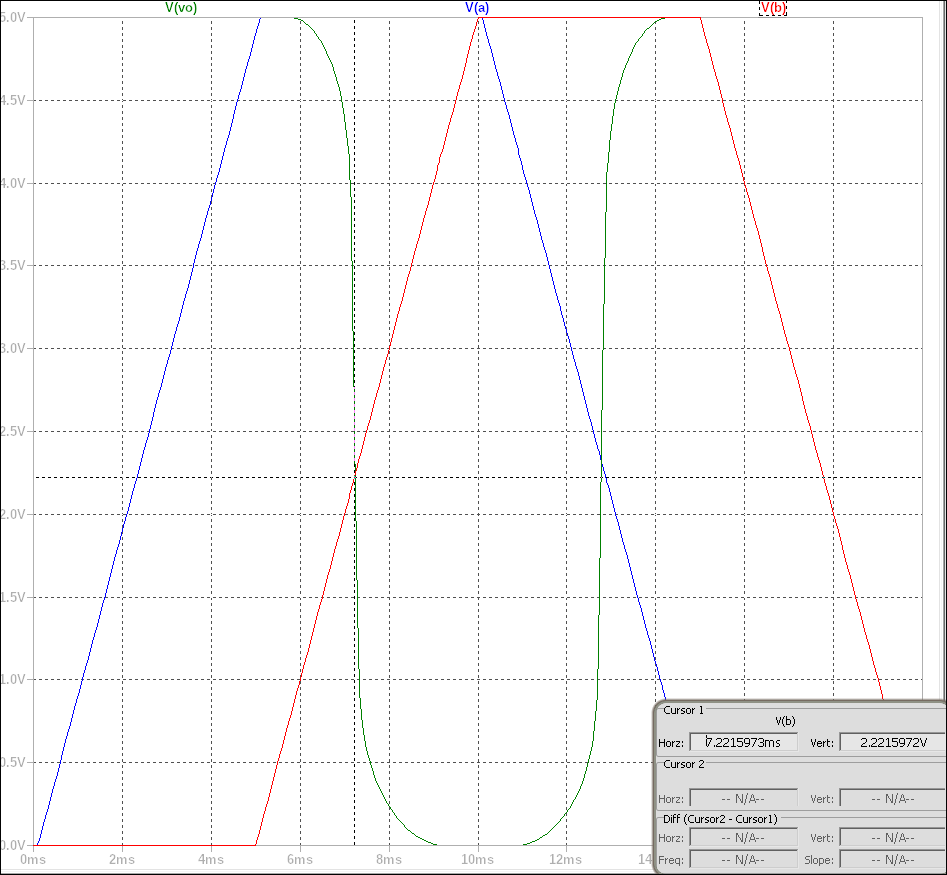
\includegraphics[width=0.8\textwidth]{Imagenes/NAND3u.png}
    \caption{Respuesta Celda NAND con $W_p = 3\mu m$}
    \label{fig:nandChoto}
\end{figure}

Pero en la simulación se encontró que se necesita $W_p = 4.8 \mu m$:

\begin{figure}[H]
    \centering
    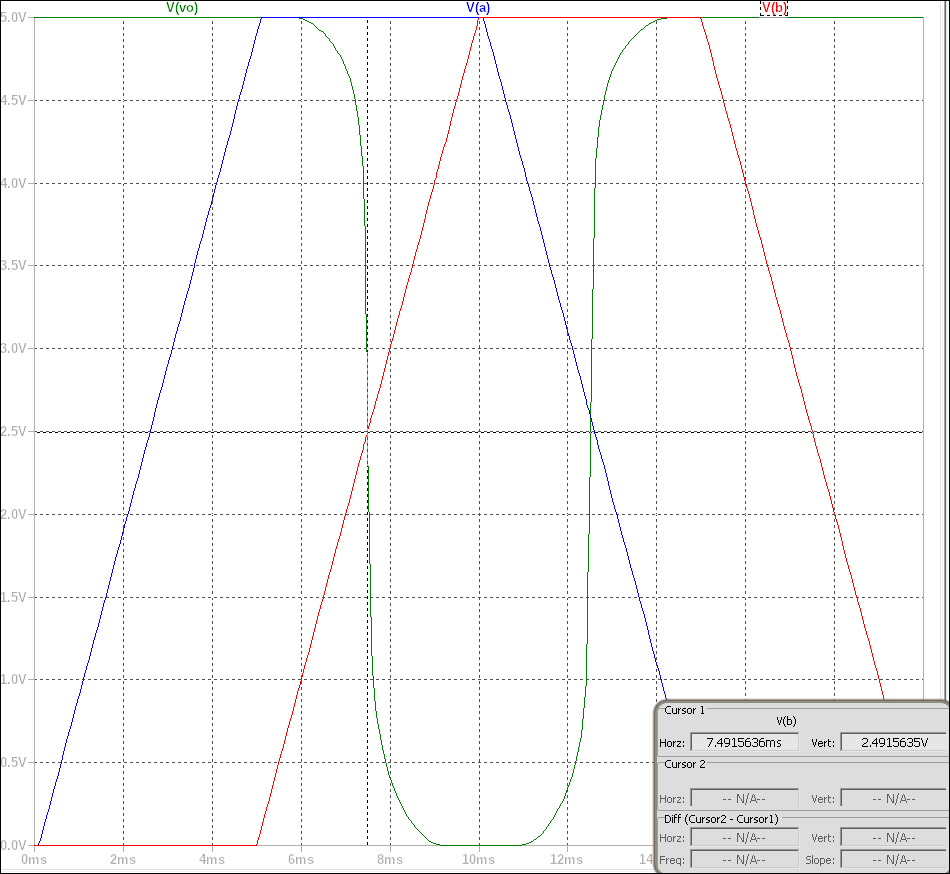
\includegraphics[width=0.8\textwidth]{Imagenes/NAND4u8.png}
    \caption{Respuesta Celda NAND con $W_p = 4.8\mu m$}
    \label{fig:nandBueno}
\end{figure}



%---------------- 7ma Seccion ----------------%
\section{FlipFlop D comparación con y sin T2 y T4}
La diferencia fundamental entre un FF-D implementado con \textit{transmission gates} (TG) y uno que no los utiliza reside en cómo se controla la transferencia y el aislamiento de la información en cada latch.

En la versión con  TG, el paso de la señal se realiza a través de interruptores bidireccionales compuestos por un NMOS y un PMOS en paralelo. Esta configuración permite una conducción prácticamente ideal de ambos niveles lógicos (‘0’ y ‘1’), evitando degradaciones de amplitud. Además, el nodo interno queda efectivamente aislado cuando el switch está abierto, lo que asegura que cada latch capture y mantenga el dato de manera robusta, incluso frente a flancos de clock no ideales o variaciones en la entrada.

Por el contrario, cuando se emplean transistores individuales gobernados por el clock, la conducción se vuelve inherentemente asimétrica: el NMOS introduce una caída en el nivel alto, mientras que el PMOS degrada el nivel bajo. A esto se suma un aislamiento menos eficiente del nodo interno, incrementando la susceptibilidad a corrientes de fuga, ruido y posibles solapamientos en las fases del clock. Como consecuencia, esta implementación presenta menor integridad de señal, pudiendo generar glitches, pérdidas del dato almacenado o incluso la propagación parcial de la entrada en condiciones en las que debería mantenerse estable.

\begin{figure}[H]
    \centering
    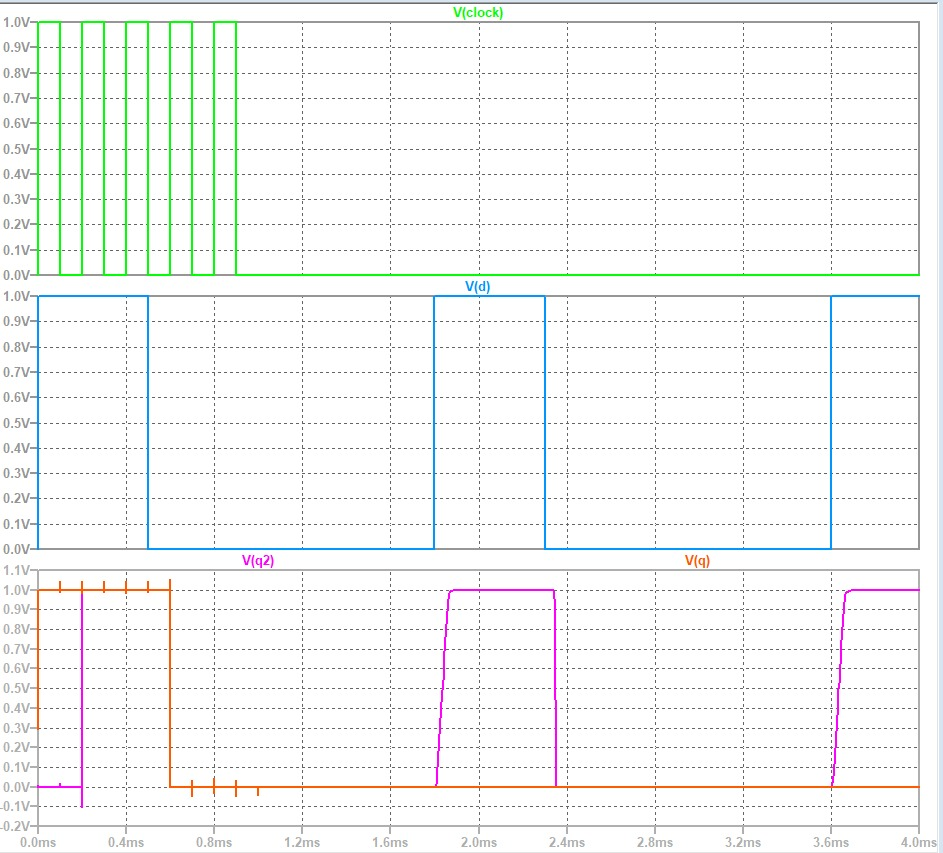
\includegraphics[width=0.8\textwidth]{Imagenes/FFMalo.jpeg}
    \caption{Comparación entre FF-D con y sin TG}
    \label{fig:FFD_comparison}
\end{figure}


Donde $V_{d}$ corresponde a la señal de entrada, $V_{(q)}$ a la salida del circuito implementado con TG, y $V_{(q2)}$ a la salida del circuito que no los utiliza.

Si se considera un clock con únicamente dos pulsos, se espera que la implementación con TG sea capaz de mantener (hold) el valor almacenado, mientras que la implementación sin estos dispositivos no debería lograrlo. Los resultados obtenidos en la simulación fueron los siguientes:

\begin{figure}[H]
    \centering
    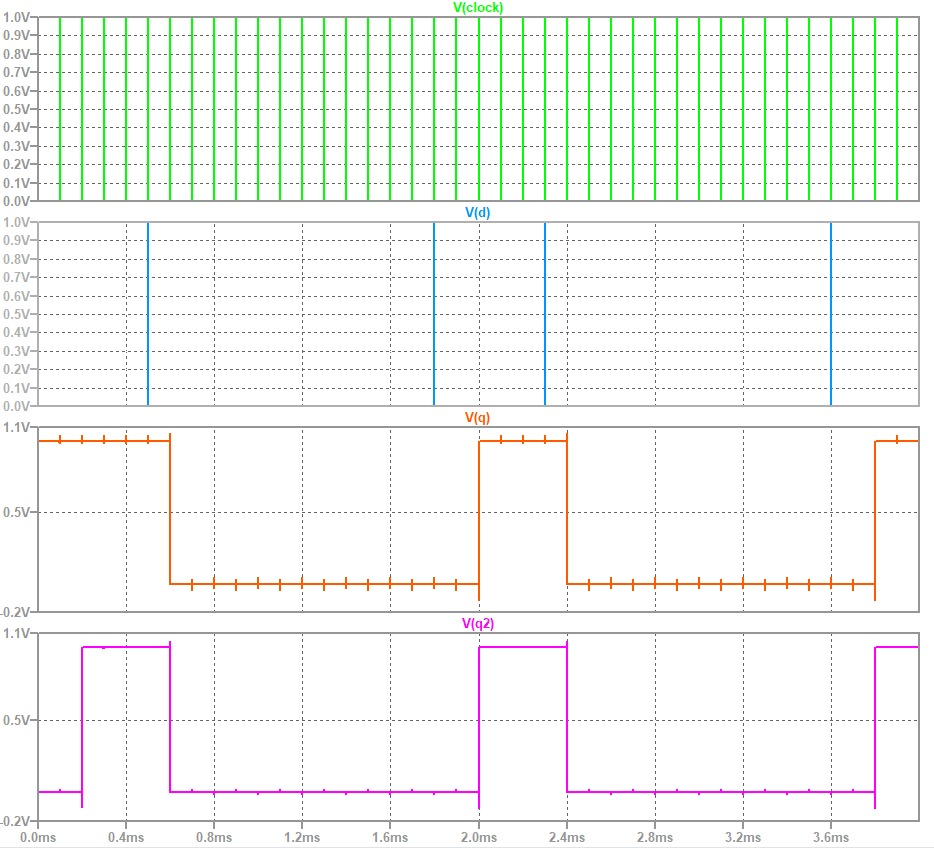
\includegraphics[width=0.8\textwidth]{Imagenes/FFBueno.jpeg}
    \caption{Simulación de FF-D con y sin TG}
    \label{fig:FFD_simulation}
\end{figure}

Cuando el clock es periódico, ambos circuitos presentan un comportamiento similar, ya que las pequeñas degradaciones de nivel lógico quedan compensadas y no afectan significativamente la conmutación. Sin embargo, cuando el clock deja de alternar, como en la simulación realizada, se pone en evidencia la diferencia estructural: en ausencia de transistores que actúen como TG, el latch no logra mantener un aislamiento adecuado y la salida pierde el dato almacenado, mientras que la implementación con TG conserva el valor sin inconvenientes.



%----------------- Conclusión ----------------%
\section{Conclusión}
Los resultados obtenidos a lo largo del trabajo permiten reinterpretar el diseño de circuitos digitales desde una perspectiva fuertemente dependiente de las no idealidades del nivel transistor. Lejos de ser un aspecto secundario, el dimensionamiento de los dispositivos CMOS condiciona de manera crítica el punto de operación de las compuertas, introduciendo asimetrías que impactan directamente en la robustez lógica y en la tolerancia al ruido.

Asimismo, el análisis dinámico pone de manifiesto que los efectos capacitivos y la interacción entre etapas no pueden ser despreciados, ya que determinan el desempeño temporal del sistema y pueden amplificar desbalances presentes en etapas previas. Esto evidencia que el diseño en cascada no es simplemente modular, sino que requiere una consideración global del circuito.

En el caso de las estructuras secuenciales, se observa que las decisiones arquitectónicas, como el uso de \textit{transmission gates}, no solo optimizan el funcionamiento, sino que resultan determinantes para garantizar la integridad de la información almacenada frente a condiciones no ideales.

En definitiva, el trabajo demuestra que el comportamiento macroscópico de los circuitos digitales está intrínsecamente ligado a fenómenos de bajo nivel, y que un diseño preciso a escala de transistor es indispensable para lograr sistemas confiables y predecibles.

%---------------- Anexo ----------------%
%\section{Anexo}
%\input{Secciones/anexo}

%---------------- Bibliografía ----------------%
%\printbibliography

%---------------- Componentes ----------------%
%\newpage
%\section{Templates}
%\input{Templates/Componentes}

\end{document}
